\documentclass[a4paper, 12pt]{article}

%%% Работа с русским языком
\usepackage{cmap}					% поиск в PDF
\usepackage{mathtext} 				% русские буквы в формулах
\usepackage[T2A]{fontenc}			% кодировка
\usepackage[utf8]{inputenc}			% кодировка исходного текста
\usepackage[russian]{babel}	% локализация и переносы

%%% Дополнительная работа с математикой
\usepackage{amsmath,amsfonts,amssymb,amsthm,mathtools} % AMS
\usepackage{icomma} % "Умная" запятая: $0,2$ --- число, $0, 2$ --- перечисление

%% Номера формул
%\mathtoolsset{showonlyrefs=true} % Показывать номера только у тех формул, на которые есть \eqref{} в тексте.

%% Шрифты
\usepackage{euscript}	 % Шрифт Евклид
\usepackage{mathrsfs} % Красивый матшрифт

%% Поля
\usepackage[left=2cm,right=2cm,top=2cm,bottom=2cm,bindingoffset=0cm]{geometry}

%% Русские списки
\usepackage{enumitem}
\makeatletter
\AddEnumerateCounter{\asbuk}{\russian@alph}{щ}
\makeatother

%%% Работа с картинками
\usepackage{graphicx}  % Для вставки рисунков
\graphicspath{{images/}{images2/}}  % папки с картинками
\setlength\fboxsep{3pt} % Отступ рамки \fbox{} от рисунка
\setlength\fboxrule{1pt} % Толщина линий рамки \fbox{}
\usepackage{wrapfig} % Обтекание рисунков и таблиц текстом

%%% Работа с таблицами
\usepackage{array,tabularx,tabulary,booktabs} % Дополнительная работа с таблицами
\usepackage{longtable}  % Длинные таблицы
\usepackage{multirow} % Слияние строк в таблице

%% Красная строка
\setlength{\parindent}{2em}

%% Интервалы
\linespread{1}
\usepackage{multirow}

%% TikZ
\usepackage{tikz}
\usetikzlibrary{graphs,graphs.standard}

%% Верхний колонтитул
\usepackage{fancyhdr}
\pagestyle{fancy}

%% Перенос знаков в формулах (по Львовскому)
\newcommand*{\hm}[1]{#1\nobreak\discretionary{}
	{\hbox{$\mathsurround=0pt #1$}}{}}

%% Мои дополнения
\usepackage{float} %Добавляет возможность работы с командой [H] которая улучшает расположение на странице
\usepackage{gensymb} %Красивые градусы
\usepackage{graphicx}               % Импорт изображений
\usepackage{caption} % Пакет для подписей к рисункам, в частности, для работы caption*

% подключаем hyperref (для ссылок внутри  pdf)
\usepackage[unicode, pdftex]{hyperref}

%%% Теоремы
\theoremstyle{plain}                    % Это стиль по умолчанию, его можно не переопределять.
\renewcommand\qedsymbol{$\blacksquare$} % переопределение символа завершения доказательства

\newtheorem{theorem}{Теорема}[section] % Теорема (счетчик по секиям)
\newtheorem{proposition}{Утверждение}[section] % Утверждение (счетчик по секиям)
\newtheorem{definition}{Определение}[section] % Определение (счетчик по секиям)
\newtheorem{corollary}{Следствие}[theorem] % Следстиве (счетчик по теоремам)
\newtheorem{problem}{Задача}[section] % Задача (счетчик по секиям)
\newtheorem*{remark}{Примечание} % Примечание (можно переопределить, как Замечание)
\newtheorem{lemma}{Лемма}[section] % Лемма (счетчик по секиям)
% % \newcommand{\eqdef}{\stackrel{\mathrm{def}}{=}}
% \newcommand{\ryad}{\sum\limits^{\infty}_{k = 0}}

% \newcommand{\R}{\mathbb{R}}
% \newcommand{\N}{\mathbb{N}}
% \newcommand{\series}{\sum\limits_{k=1}^{\infty}}
% \newcommand{\useries}{\sum\limits_{k=1}^{\infty} u_k}
% \newcommand{\useriesl}{\sum\limits_{k=1}^{\infty} u_k < \infty}
% \newcommand{\useriese}{\sum\limits_{k=1}^{\infty} u_k = \infty}
% \newcommand{\auseries}{\sum\limits_{k=1}^{\infty} |u_k|}
% \newcommand{\auseriesl}{\sum\limits_{k=1}^{\infty} |u_k| < \infty}
% \newcommand{\auseriese}{\sum\limits_{k=1}^{\infty} |u_k| = \infty}
% \newcommand{\sn}{\sum\limits_{k=1}^{n} u_k}

% \renewcommand {\ge}{\geqslant}
% \renewcommand {\le}{\leqslant}
% \renewcommand {\geq}{\geqslant}
% \renewcommand {\leq}{\leqslant}
% \renewcommand {\epsilon}{\varepsilon}

\begin{document}

    \newcommand{\HRule}{\rule{\linewidth}{0.7mm}} % Defines a new command for the horizontal lines, change thickness here
	
	\begin{center}
		\large\textbf{Московский Физико-Технический Институт}\\ % Name of your university/college
		\large\textbf{(государственный университет)}
	
		\vfill
		
		\Large Лабораторная работа по курсу общей физики № *labnum*\\[0.5cm] % Preambule of your document title
		
		
		\HRule
		\\[0.4cm]
		{ \huge \bfseries *name of your labwork*}% Title of your document
		\\[0.4cm] 
		\HRule
		\\[0.5cm]
		
		\ \\
	\textbf{\large Автор:} \\	
	\large *your name* *groupname*\\ % Your name and something more, your group num for example
		\vfill
		\hspace*{-0.8 cm}
\includegraphics[width=100 pt]{frkt_logo}\\ % logo of your  company/university/college
		\large Долгопрудный, 2021 % location and year
	\end{center}

\newpage
\setcounter{page}{2}
\fancyfoot[c]{\thepage}
\fancyhead[L] {Работа № *labnum*} % some information in page header
\fancyhead[R]{}
        \section*{Теоретическая часть.}

    \begin{figure}[h!]
        \centering
        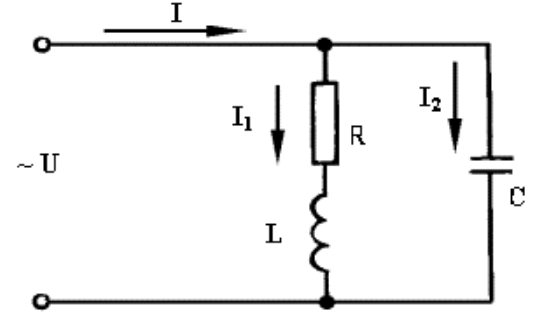
\includegraphics[scale = 0.3]{схема_цепи.png}
        \caption{Схема цепи}
    \end{figure}

    \noindent В этой схеме общим параметром для двух ветвей является напряжение $U$. 
    Первая ветвь -- индуктивная катушка -- обладает активным сопротивлением $R$ и индуктивностью $L$. 
    Результирующее сопротивление $Z_1$ и ток $I_1$ определяются по формуле:

    \begin{equation*}
        Z_1 = \sqrt{R^2 + X_L^2}
    \end{equation*}
    где $X_L = \omega L$.
    \begin{equation*}
        I_1 = \frac{U(t)}{Z_1}
    \end{equation*}

    \noindent Ток в ветви отстает по фазе от напряжения на угол

    \begin{equation*}
        \varphi_1 = \arctan \frac{R}{X_L}
    \end{equation*}

    \begin{figure}[h!]
        \centering
        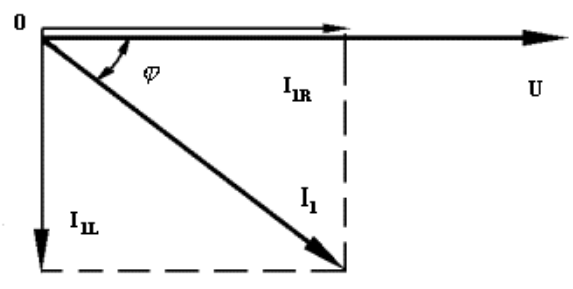
\includegraphics[scale = 0.3]{фазовая_диаграмма1.png}
        \caption{фазовая диаграмма}
    \end{figure}

    \noindent Во вторую ветвь включен конденсатор. Его сопротивление

    \begin{equation*}
        Z_2 = X_C = \frac{1}{\omega L}
    \end{equation*}

    \begin{equation*}
        \frac{U(t)}{Z_2}
    \end{equation*}

    \noindent Этот ток опережает по фазе напряжение на $\frac{\pi}{2}$.
    Для определения тока I в неразветвленной части цепи воспользуемся формулой:

    \begin{equation*}
        I = \sqrt{I_R^2 + (I_L - I_C)^2}
    \end{equation*}

    \begin{figure}[h!]
        \centering
        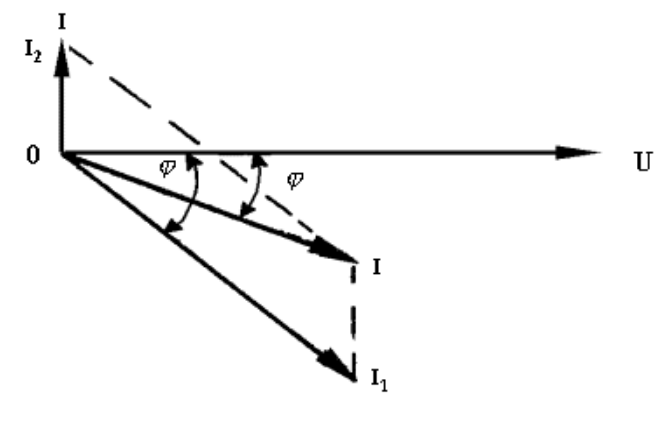
\includegraphics[scale = 0.3]{фазовая_диаграмма2.png}
        \caption{фазовая диаграмма}
    \end{figure}

    \noindent Угол сдвига между током и напряжением обозначим буквой $\theta$.

    \noindent Возможен режим работы схемы, когда $\theta = 0$, 
    т.е. ток в неразветвленной части цепи I будет иметь активный характер. 
    Произойдет это в случае, когда $I_L = I_C$, 
    т.е. при равенстве реактивных составляющих тока в ветвях.

    \begin{figure}[h!]
        \centering
        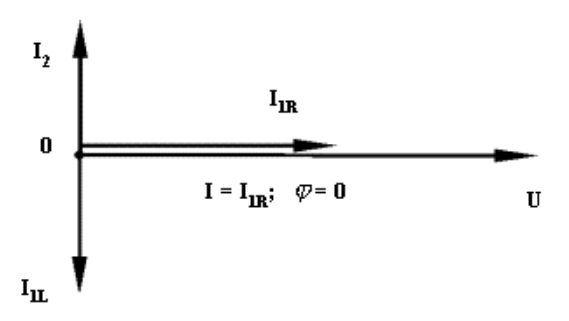
\includegraphics[scale = 0.3]{фазовая_диаграмма3.png}
        \caption{фазовая диаграмма}
    \end{figure}

    \noindent Такой режим называется резонансом токов.

    \noindent Найдем условие, при котором возникает резонанс токов.
    Как видно из фазовой диаграммы:

    \begin{equation*}
        I_2 = I_1 \sin \varphi \Rightarrow
    \end{equation*}

    \begin{equation*}
        \sin \varphi = \frac{\omega L}{\sqrt{R^2 + (\omega L)^2}}
    \end{equation*}

    \begin{equation*}
        \cos \varphi = \frac{R}{\sqrt{R^2 + (\omega L)^2}}
    \end{equation*}

    Таким образом, условие резонанса токов:

    \begin{equation*}
        \omega = \omega_0 = \frac{1}{\sqrt{LC}}
    \end{equation*}

    Вычислим теперь амплитуду полного тока при резонансе.

    \begin{equation*}
        I = I_1 \cos \varphi
    \end{equation*}

    \begin{equation*}
        I = \frac{U_0}{\sqrt{R^2 + (\omega L)^2}} \cdot \frac{R}{\sqrt{R^2 + (\omega L)^2}} \approx \frac{U_0 R C}{L}
    \end{equation*}

    Тогда выразим резонансное напряжение:

    \begin{equation*}
        R_{\text{рез}} = \frac{U_0}{I} = \frac{L}{R C}
    \end{equation*}

    \noindent Отношение резонансного сопративления $R_{\text{рез}}$ контура
    к его активному сопративлению равно квадрату добротности контура.

    \begin{equation*}
        Q^2 = \frac{R_{\text{рез}}}{R}
    \end{equation*}

    \section*{Подготовка.}

    \noindent \textbf{В работе используются:} изучение параллельной цепи переменного тока, наблюдение резонанса токов.
	
	\noindent \textbf{Цель работы:} лабораторный автотрансформатор (ЛАТР),
    разделительный понижающий трансформатор, ёмкость, дроссель с переменной индуктивностью, три амперметра, вольтметр, реостат, электронный осциллограф, омметр, мост переменного тока.
	
    \hfill

    \noindent \textbf{Эксперементальная установка.}

    \noindent Схема экспериментальной установки
    приведена на рисунке. Напряжение от сети (220 В, 50 Гц) с помощью ЛАТРа через понижающий трансформатор Тр подаётся на параллельный
    контур, содержащий конденсатор ($C$ = 120 мкФ) и катушку, индуктивность которой зависит от глубины погружения сердечника. Полный ток
    в цепи измеряется с помощью многопредельного амперметра $A_1$; для измерения токов в $L$ и $C$ ветвях используются два одинаковых амперметра
    $A_2$ и $A_3$; напряжение на контуре контролируется электронным вольтметром V. Последовательно с контуром включён резистор $r$ -- реостат с полным сопротивлением $\simeq 100$ Ом.

    \begin{figure}[h!]
        \centering
        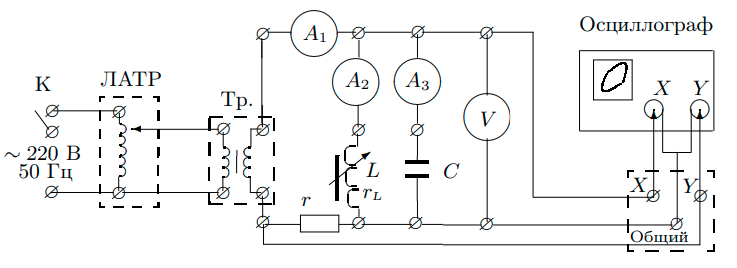
\includegraphics[scale = 0.6]{Схема_эксперементальной_установки.png}
        \caption{}
    \end{figure}

    \hfill

    \noindent Для наблюдения за сдвигом фаз между полным током и напряжением
    на контуре используется осциллограф. Сигнал, пропорциональный току,
    снимается с резистора $r$ и подаётся на вход $Y$ осциллографа. На вход $X$
    подаётся напряжение непосредственно с контура. При наличии сдвига
    фаз между этими напряжениями на экране виден эллипс, а при нулевом
    сдвиге фаз эллипс вырождается в прямую. 
    
    %========================================================================================================================
    
    \section{Обработка данных}
	
	
	Снимем зависимость резонансной частоты от емкости конденсатора. Входное напряжение $U_0 = 100$ мВ. Резонансную частоту будем измерять двумя способами: в режиме развертки и по фигурам Лиссажу (в режиме резонанса наблюдаем вырожденный эллипс).\\
	$\nu_{\text{рез1}}$ -- частота по фигурам Лиссажу, $\nu_{\text{рез2}}$ -- по развертке.
	
	\begin{table}[h!]
		\begin{center}
			\begin{tabular}{|c|c|c|c|c|c|c|}
				\hline
				$U_0$ мВ & $U_c$ мВ & $\nu_{\text{рез1}}$ кГц & $\nu_{\text{рез2}}$ кГц & $T$ мкс & $(T/2 \pi)^2$ & $C$ нФ \\ \hline
				100      & 286      & 23,77                   & 23,56                   & 42      & 44,7          & 47,9   \\ \hline
				100      & 230      & 21,5                    & 21,25                   & 47      & 56,0          & 57,4   \\ \hline
				100      & 192      & 19,98                   & 19,72                   & 51      & 66,0          & 66,7   \\ \hline
				100      & 152,5    & 18,07                   & 17,74                   & 56      & 79,5          & 82,1   \\ \hline
				100      & 124      & 16,45                   & 16,19                   & 62      & 97,0          & 99,6   \\ \hline
			\end{tabular}
		\end{center}
	\end{table}
	
	Построим график зависимости величины $(T/2 \pi)^2$ от емкости.
	
	\begin{figure}[h!]
		\centering
		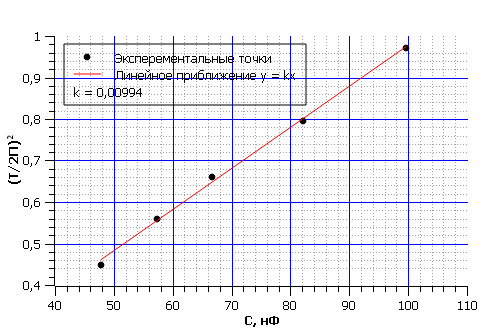
\includegraphics[scale = 1]{T_C_.jpg}
		\caption{}
	\end{figure}
	
	В соответствии с формулой $T = 2 \pi \sqrt{L C}$ по угловому коэффициенту найдем индуктивность.
	
	\begin{center}
		\fbox{$L = 0,01$ мГн}
	\end{center}

	Снимем амплитудно-частотную характеристику для двух значений емкости $C_1 = 47,9$ нФ ($\nu_{\text{рез}} = 235,6$ кГц) и $C_2 = 99,6$ нФ ($\nu_{\text{рез}} = 235,6$ кГц). Входное напряжение $U_0 = 100$ мВ.
	
	\newpage
	
	\begin{table}[h!]
		\begin{center}
			\begin{tabular}{|c|c|c|}
				\hline
				$\nu$, кГц & $U_c$, мВ & $A = \sqrt{2} U_c$ \\ \hline
				14,15      & 42,0      & 59,39  \\ \hline
				16,45      & 44,2      & 62,50  \\ \hline
				18,83      & 52,7      & 74,53  \\ \hline
				21,22      & 82,8      & 117,09 \\ \hline
				22,35      & 131,0     & 185,26 \\ \hline
				23,00      & 207,0     & 292,74 \\ \hline
				23,56      & 286,0     & 404,47 \\ \hline
				24,05      & 227,0     & 321,03 \\ \hline
				24,78      & 120,0     & 169,71 \\ \hline
				25,90      & 58,0      & 82,024 \\ \hline
				28,20      & 26,5      & 37,48  \\ \hline
				31,00      & 10,0      & 14,14  \\ \hline
			\end{tabular}
		\end{center}
	\end{table}

	\begin{table}[h!]
		\begin{center}
			\begin{tabular}{|c|c|c|}
				\hline
				$\nu$, кГц & $U_c$, мВ & $A = \sqrt{2} U_c$ \\ \hline
				10,68      & 47,0      & 66,47  \\ \hline
				12,40      & 47,1      & 66,61  \\ \hline
				14,20      & 51,6      & 72,97  \\ \hline
				16,00      & 71,6      & 101,26 \\ \hline
				17,80      & 99,6      & 140,86 \\ \hline
				19,56      & 36,7      & 51,90  \\ \hline
				21,30      & 9,7       & 13,72  \\ \hline
			\end{tabular}
		\end{center}
	\end{table}

	\newpage

	\begin{figure}[h!]
		\centering
		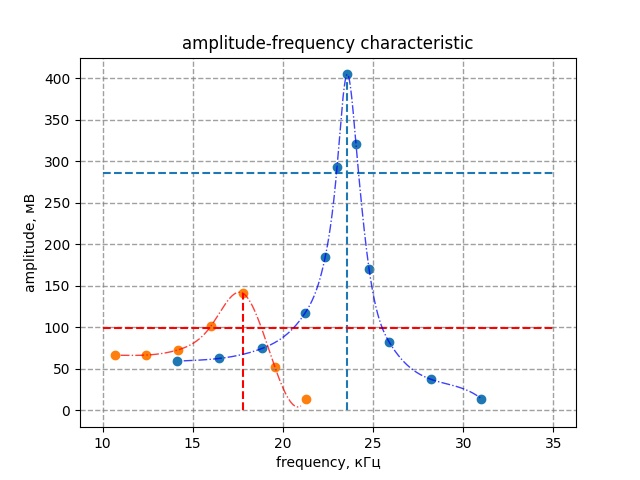
\includegraphics[scale = 1]{quality_factor.jpg}
		\caption{График добротности}
	\end{figure}
	
\end{document}